\documentclass{article}
\usepackage{tikz}
\usetikzlibrary{arrows.meta} 
\usetikzlibrary{shapes.geometric} 
\usetikzlibrary{decorations,decorations.pathreplacing}
\usetikzlibrary{shadings}

\definecolor{cellcolor}{RGB}{232, 239, 255}

\usepackage[utf8]{inputenc}
\usepackage{geometry}

\geometry{
    left=1cm,
    right=1cm,
    top=1.5cm,
    bottom=2.5cm
}

\usepackage{setspace}
\usepackage{xcolor}

\begin{document}

\begin{Large}
    \begin{singlespace}
       \begin{center}
        \textbf{Animal Cell - Template} \\
        Version 1.0.0
       \end{center} 
    \end{singlespace}
\end{Large}

\vspace*{10mm}

\begin{center}
    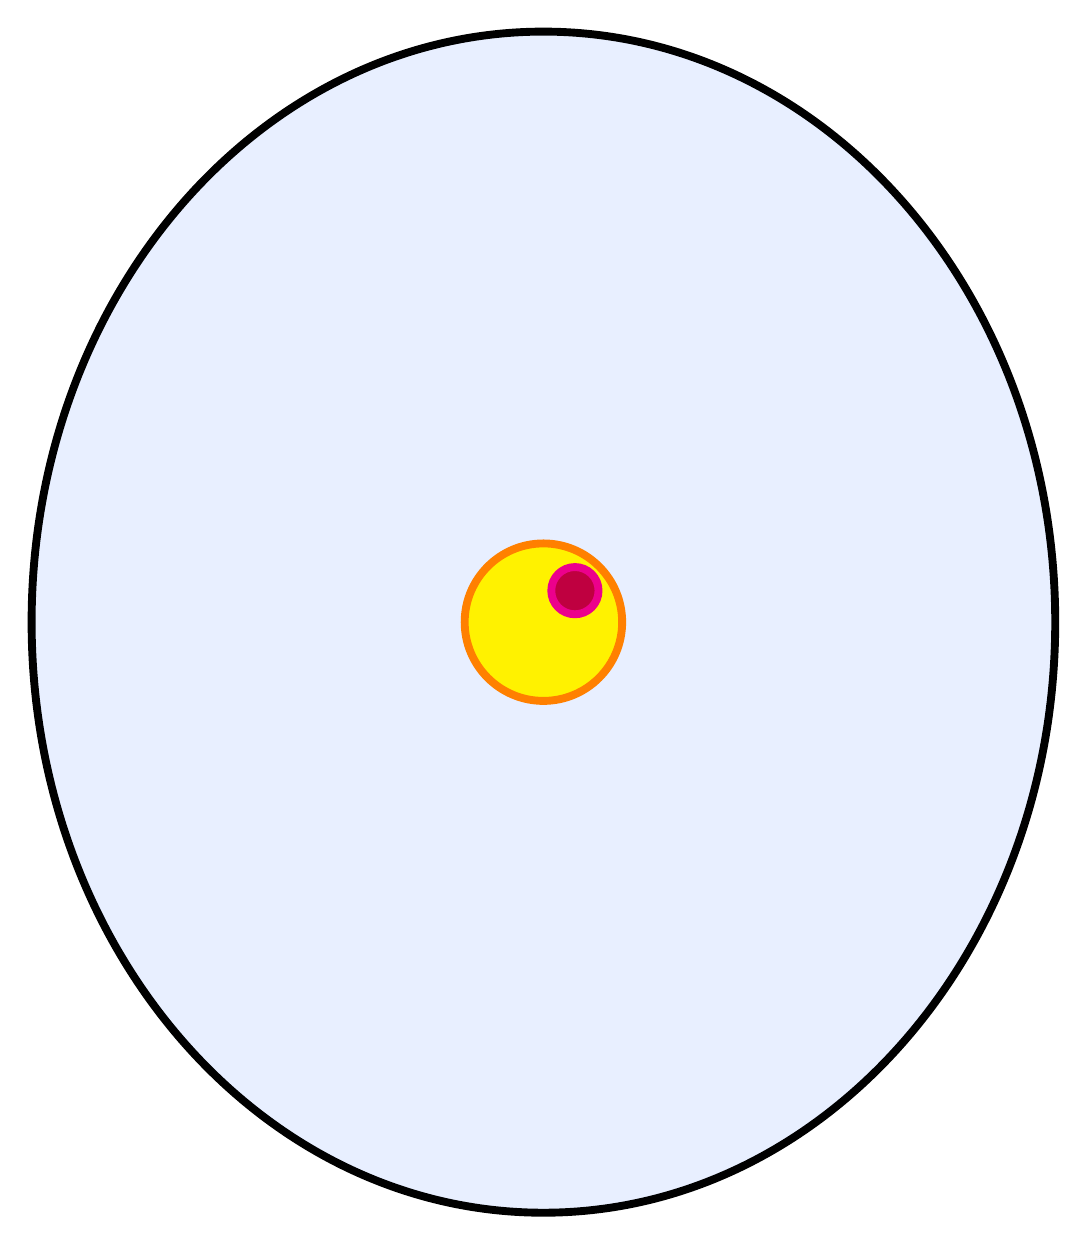
\begin{tikzpicture}
        \node[shape=ellipse,
              draw=black,
              very thick,
              line width=1mm,
              fill=cellcolor,
              text=black,
              rotate=90,
              minimum height = 13cm,
              minimum width = 15cm] at (0,0) {};
        \node[shape=circle,
              draw=orange,
              very thick,
              line width=1mm,
              fill=yellow,
              text=black,
              rotate=90,
              minimum height = 2cm,
              minimum width = 2cm] at (0,0) {};
        \node[shape=circle,
              draw=magenta,
              very thick,
              line width=1mm,
              fill=purple,
              text=black,
              rotate=90,
              minimum height = 0.6cm,
              minimum width = 0.6cm] at (0.4,0.4) {};
    \end{tikzpicture}
\end{center}

\end{document}